\documentclass{article}
\usepackage{graphicx} % Required for inserting images
\usepackage[T2A] {fontenc} 
\usepackage{graphicx}
\graphicspath{ {images/} }

\title{Design document}
\author{Кирилл Бобровицкий, Максим Бобровицкий\\
Даниил Смирнов, Руслан Мухаметшин, Артем Антонов}
\date{November 2024}

\begin{document}

\maketitle

\tableofcontents
\newpage

\section{Введение}


\newpage

\section{Концепция}
\subsection{Введение}
\noindent\textit{\textbf{\underline{Некогда процветающий край, ныне покрытый тенью проклятия…}}}
Междугорье, регион, скрытый за высокими горами, был местом гармонии и изобилия, пока жрецы злого бога не попытались бросить вызов самой жизни.  
Вы — последний не заражённый, пробудившийся в сердце этой тьмы. Ваша цель — уничтожить последователей злого бога, поддерживающих проклятие, пока Междугорье окончательно не рухнуло.

\subsection{Жанр и аудитория}
Жанр: рогалик(rogue-like), платформер, приключенческий экшн.\\  
Аудитория: 12+

\subsection{Основные особенности игры}
\begin{itemize}
\item Междугорье совмещает в себе два популярнейших жанра - рогалик и  платформер. Исследование локаций оформлено в виде рогалика, но чтобы перейти в следующую локацию необходимо пройти подземелье текущей локации, в котором игра будет организована в виде платформера. 

\item Комнаты и расположение предметов внутри локаций генерируются процедурно, обеспечивая высокую реиграбельность. Каждый запуск игры будет уникальным. 

\item Финальная битва с боссом станет уникальным и динамичным испытанием, использующим возможности нейронных сетей. Босс не будет просто следовать заранее заданному алгоритму - он будет обладать адаптивным искусственным интеллектом, способным обучаться в режиме реального времени. Во время боя нейросеть будет анализировать действия игрока: выбор атак, уклонений, использование предметов и тактические решения. На основе полученных данных ИИ босса будет динамически корректировать свои действия.
\end{itemize}

\subsection{Описание игры}
Основная часть игры  происходит  в виде двухмерного шутера с видом сверху. Игроку необходимо достичь финальной комнаты, по пути разбираясь с мобами и находя себе снаряжение. Снаряжение состоит из основного оружия, которое наносит урон мобам, дополнительного оружия, которое можно использовать через определенное время и аксессуара, который даёт определенный баф.
В игре нет деления на уровни, действие происходит на одной большой карте, которая поделена на несколько локаций, которые в свою очередь поделены на "комнаты". 
У каждой локации есть свой отличающийся от остальных стиль и набор мобов. В каждой из локации обязательно присутствуют комнаты: Руины Храма, где можно восстановить здоровье или получить от темных сил случайное оружие, Разрушенный магазин, где можно купить у его хранителя снаряжение.
Также у каждой локации есть свое подземелье, вход в которое находится в одной из комнат. В подземелье можно найти минибоса, после победы над которым можно получить особый элемент снаряжения. Также в одной из комнат подземелья находится определенный ключ для перехода на следующую локацию. После прохождения локации игрока ждёт битва с боссом. Победа над ним заканчивает игру.
При повторном прохождении игрок получит новый игровой опыт, так как элементы снаряжения появляются в мире случайным образом и боевая механика босса зависит от действий игрока.

\subsection{Предпосылки создания}
Личностный рост: Путь главного героя от простого жителя Междугорья до спасителя мира может стать источником глубокого личностного роста и трансформации персонажа. Это привлечет игроков, которые ценят развитие персонажей и сложные сюжеты.
Идентификация с героем: Уникальное положение главного героя как последнего незараженного человека делает его особенно привлекательным для игроков, позволяя им почувствовать себя частью чего-то великого и важного.
Эмоциональный резонанс: История главного героя, его борьба и жертвы ради спасения мира вызывают сильные эмоции у игроков, что способствует более глубокому погружению в игру.

\subsection{Платформа}

\begin{table}[h]
    \centering
    \caption{Системные требования}
    \begin{tabular}{|l|l|l|}
        \hline
        \textbf{Платформа} & \textbf{Минимальные требования} & \textbf{Рекомендуемые требования} \\ \hline
        Windows & 
        \begin{tabular}[c]{@{}l@{}}OS: Windows 7+ \\ Процессор: Intel i3+ \\ Оперативная память: 2 ГБ \\ Графика: Nvidia 450 GTS+\\ Хранилище: 500 МБ \\ Дополнительно: DirectX 9.1+ или OpenGL3.2+\end{tabular} & 
        \begin{tabular}[c]{@{}l@{}}OS: Windows 10+ \\ Процессор: Intel i5+ \\ Оперативная память: 4 ГБ \\ Графика: Nvidia GTX 660+ \\ Хранилище: 500 МБ \\ Дополнительно: DirectX 11+\end{tabular} \\ \hline
        
        Mac & 
        \begin{tabular}[c]{@{}l@{}}OS: Mavericks 10.9\\ Оперативная память: 2 ГБ\\ Графика: OpenGL 3.2+\\ Хранилище: 500 МБ\end{tabular} & 
        \begin{tabular}[c]{@{}l@{}}OS: Catalina 10.15+\\ Оперативная память: 4 ГБ\\ Графика: OpenGL 4.1+\\ Хранилище: 500 МБ\end{tabular} \\ \hline
        
        Linux & 
        \begin{tabular}[c]{@{}l@{}}Оперативная память: 2 ГБ \\ Графика: Nvidia 450 GTS+ \\ Хранилище: 500 МБ \\ Дополнительно: OpenGL 3.2+\end{tabular} & 
        \begin{tabular}[c]{@{}l@{}}Оперативная память: 4 ГБ \\ Графика: Nvidia GTX 660+\\ Хранилище: 500 МБ\end{tabular} \\ \hline
    \end{tabular}
    \label{tab:dead_cells_requirements}
\end{table}

\section{Функциональная спецификация}
\subsection{Принципы игры}
\subsubsection{Суть игрового процесса}
Процесс игры заключается в зачистке комнат для получения лучшего снаряжения и нахождения подземелье (рогалик), в котором надо найти и убить босса(платформер), после чего идёт переход на следующий этап. Всего в игре три этапа и три соответствующих им подземелья и финальная локация - замок (платформер). С каждой новой локации характеристики врагов увеличиваются относительного предыдущего. Реиграбильность обеспечивается за счёт процедурной генерации и механики ИИ(3.5).
\begin{figure}[h]
    \centering
    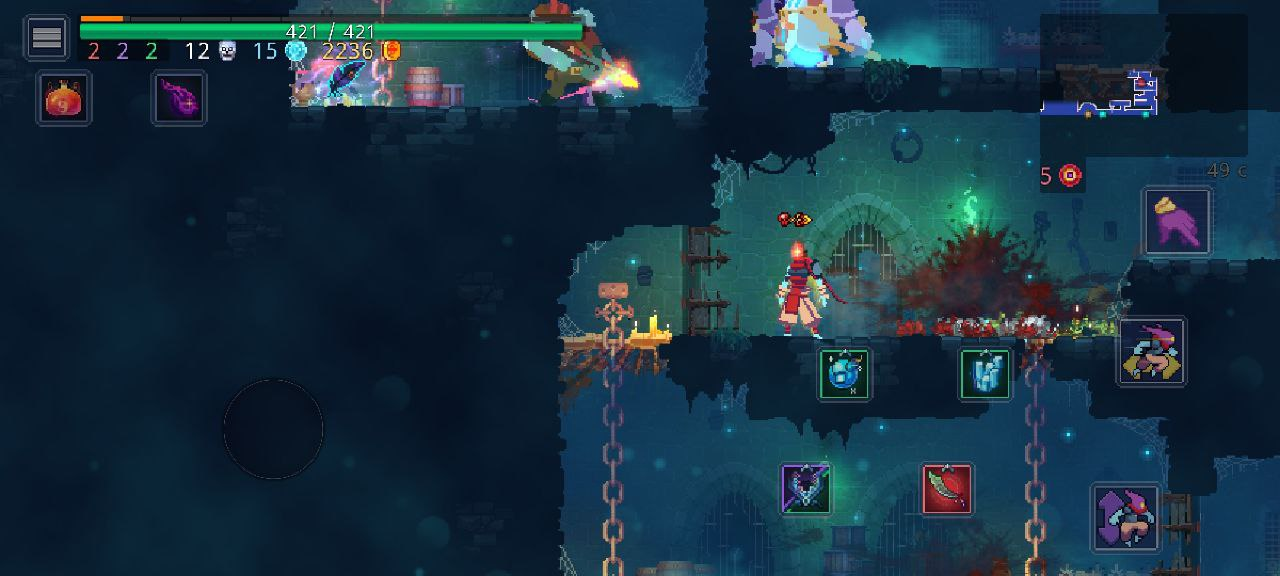
\includegraphics[width=1\textwidth]{primerP}
    \caption{Пример рогалика}
\end{figure}
\begin{figure}[h]
    \centering
    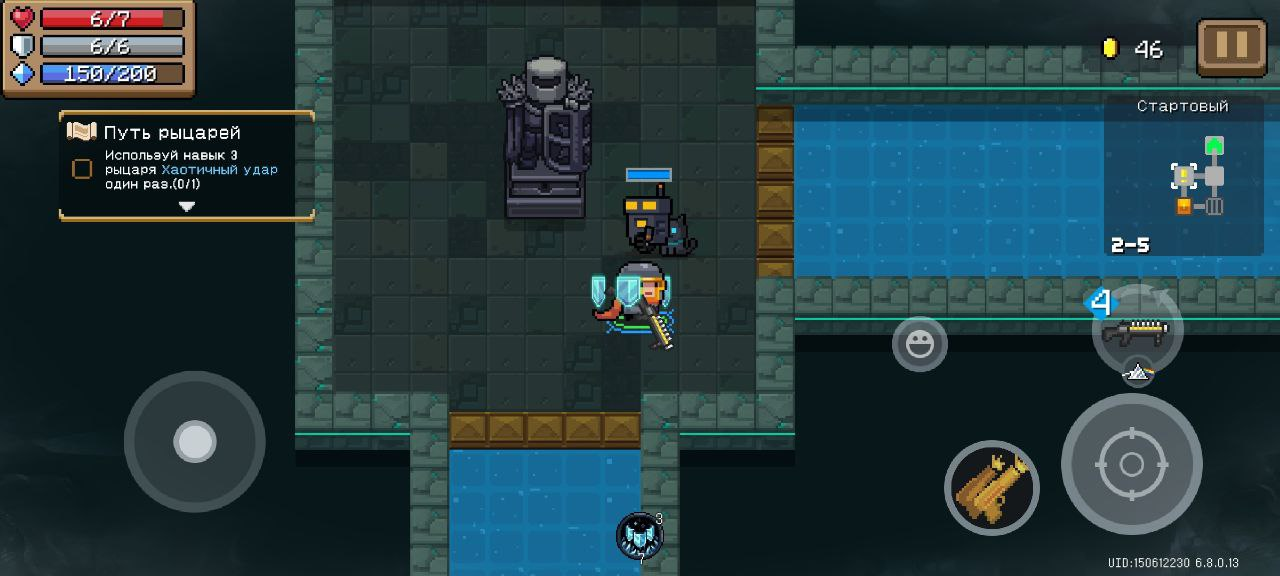
\includegraphics[width=1\textwidth]{primerR}
    \caption{Пример платформера}
\end{figure}
\subsubsection{Ход игры и сюжет}
В начале показывается как главный герой антропоморфное бесформенное существо в мешковатом костюме с капюшоном, после чего появляется гид факелок, который объясняет текущую ситуацию в междугорье и что ему нужно найти и устранить силу поддерживающую проклятье. Дальше игрок двигается вперед по этапам с подсказками гида, основная история локаций и их героев лежит в описании внутриигровых предметов и книгах. Схема прохождения локаций такая: найти первый ключ в первой половине локации, потом найти ключ от подземелья, дальше пройти его и перейти на следующий этап. В финальной локации герои необходимо преодолеть врагов и найти локацию тронного зала, в котором нужно решить  несколько головоломок и (spoiler alert) после чего встретиться с финальным сосредоточением зла - самим собой.
\subsection{Физическая модель}
Физическая модель игры основана на законах движения и взаимодействия объектов, характерных для средневекового мира. Персонажи передвигаются с учётом массы, инерции и силы трения. Ближний бой включает реалистичную симуляцию ударов холодным оружием, блоков и парирований, где учитываются сила удара, угол столкновения и тип материала оружия и брони. Элементы окружения, такие как падение камней или разрушение деревянных конструкций, происходят под воздействием гравитации и силы удара, создавая динамическую игровую среду.
\subsection{Персонаж игрока}
Для игры roguelike характерным персонажем может быть отважный исследователь подземелий. Аватар игрока может быть представлен в виде смельчака в ржавой броне, с рюкзаком через плечо и факелом в руках, готового идти на поиски сокровищ и приключений. Его лицо может быть скрыто под капюшоном или шлемом, добавляя ауру таинственности.
\subsection{Элементы игры}
*Все приведённые картинки лишь примеры. Реальная игра может сильно отличаться.
\subsubsection{Враги}
Указаны базовые значения.
\begin{itemize}
\item Чечик – в этих безмозглых монстров превратились самые рядовые жители Междугорья. По одиночке не очень сильны – 200 HP и 30 очков урона в близи, но в толпе представляют большую опасность.
\item Стражник Мглы – когда-то бравые защитники рубежей превратились в бездушные смертоносные машины, вооруженные луками. 150 HP и 60 очков дальнего урона.
\item Линчеватель – земские волшебники, к которым раньше обращались за помощью жители, под влиянием сил тьмы обратились в злобных колдунов, творящих хаос на своем пути. 150 HP и 40 очков дальнего урона, на расстоянии меньше шести блоков урон возрастает до 75. 
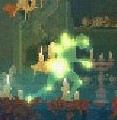
\includegraphics[width=0.3\linewidth]{dd_chehcik.jpg}\hspace{0.5cm}
\includegraphics[width=0.22\linewidth]{dd_luchnik.jpg}\hspace{0.5cm}
\includegraphics[width=0.2\linewidth]{images/dd_mag.jpg}
\end{itemize}
\subsubsection{Строения}
\begin{itemize}
\item Руины Храма - Развалины места, в которое раньше стекались люди чтобы просить высшие силы о разной помощи: кто-то молил у богов о поражающей силе, кто-то о чудесном выздоровлении, кто-то о безграничной удаче, кто-то о рождении ребёнка. В общем, Храмы раньше были центром притяжения во всех частях Междугорья, но после катастрофы опустели даже они. Боги растеряли свою паству, однако всё ещё способны одарить своим благословлением одинокого прихожанина.
В ныне пустующем здании стоит большая статуя, представляющая собой двух сросшихся человекоподобных существ, одно из них, с правой стороны, явно доброе божество, другое, с левой, – явно злое. Если поклониться доброму, то здоровье персонажа полностью восстановится, если поклониться злому – в комнате появится случайный элемент снаряжения с особым усилением. 
\item Разрушенный Магазин – покосившееся здание когда-то аккуратного и чистого заведения. Когда Междугорье процветало, один предприимчивый человек создал крупную компанию, получившую от властей право продавать почти всё.  Магазины этой компании стабильно работали во всех регионах, пока не случился катаклизм. Но владельцу было легче преодолеть смерть, чем допустить то, что из его магазинов что-то возьмут бесплатно…
В Разрушенном Магазине появляются по одному случайному экземпляру каждого элемента снаряжения. Приобрести снаряжение можно у Хранителя Магазина за монеты, которые выпадают с мобов.\\
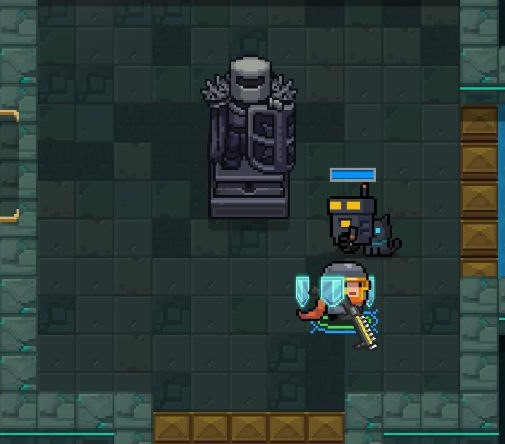
\includegraphics[width=0.3\linewidth]{images/dd_hram.jpg}\hspace{0.5cm}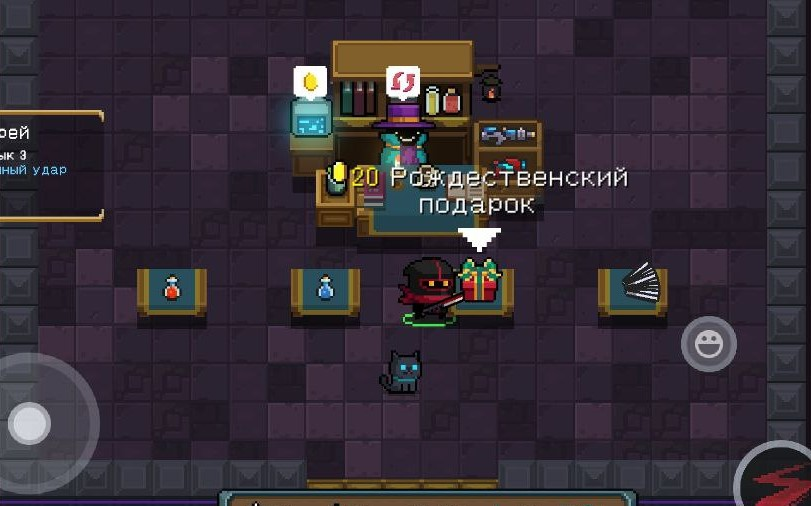
\includegraphics[width=0.4\linewidth]{images/dd_store.jpg}
\end{itemize}
\subsubsection{Оружие и другие элементы снаряжения}
У каждого элемента снаряжения есть три редкости – обычная, редкая и легендарная. Сначала приведены изображения оружия в платформере, а затем - в рогалике.
\paragraph{Основное оружие}
\begin{itemize}
\item Оружие ближнего боя.
Представляет собой старый добрый меч. Высокая скорость, наносит в ближнем бою 50/75/100 единиц урона в зависимости от редкости.\\

\includegraphics[width=0.23\linewidth]{images/dd_mech.jpg}\hspace{0.5cm}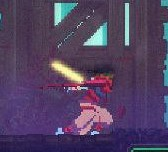
\includegraphics[width=0.3\linewidth]{images/dd_mech21.jpg}\hspace{0.5cm}
\includegraphics[width=0.3\linewidth]{images/dd_mech22.jpg}
\item Магическое оружие.
Магические посохи, эффективные на средних дистанциях. Средняя скорость, на расстоянии не большем чем пять блоков наносит 75/100/125 единиц урона, на более дальнем - 40/65/900 в зависимости от редкости.\\

\includegraphics[width=0.23\linewidth]{images/dd_posoh.jpg}
\item Дальнобойное оружие.
Длинные луки, излюбленное оружие стражников, хорошо подходит для дальних дистанций.  Низкая скорость, наносит 100/130/160 единиц урона в зависимости от редкости.\\
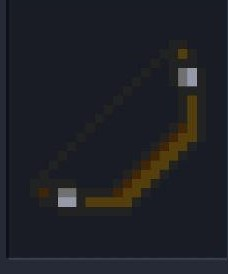
\includegraphics[width=0.2\linewidth]{images/dd_luk.jpg}\hspace{0.5cm}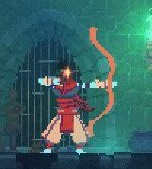
\includegraphics[width=0.22\linewidth]{images/dd_luk2.jpg}
\end{itemize}
\paragraph{Взрывчатка}
\begin{itemize}
\item Граната. Она наносит 40/50/60 единиц мгновенного урона в р в зависимости от редкости
\item Коктейль Молотовcкого. Когда-то самый популярный напиток, превратившийся в зажигательную смесь. Наносит 20/30/40 единиц мгновенного урона и затем наносит противнику ещё 5/7/10 единиц урона раз в секунду на протяжении 4 секунд в зависимости от редкости.
\item Склянка с морозом. Наносит 30/40/50 единиц мгновенного урона и замораживает врагов на 3/4/5 секунд(ы) в зависимости от редкости.

\end{itemize}
\paragraph{Аксессуары}
\begin{itemize}
\item Кольцо с рубином. Увеличивает здоровье на 10/20/30 процентов в зависимости от редкости.
\item Кольцо с изумрудом. Увеличивает скорость на 10/20/30 процентов в зависимости от редкости.
\item Кольцо с сапфиром. Увеличивает урон на 10/20/30 процентов в зависимости от редкости.
\item Обручальное кольцо. Непростое украшение, нет бонуса.
\end{itemize}
\subsubsection{NPC}
\begin{itemize}
\item Хранитель магазина. Жадный дух. Который за ваши кровные продаст вам всё что угодно.  
\item Факелок. Добродушное таинственное существо, которое рассказывает главному герою о всех изменениях в Междугорье после катаклизма.
\end{itemize}
\subsubsection{Предметы}
\begin{itemize}
\item Междугорский рульден – основная валюта междугорья, оставшаяся в карманах зараженных жителей.
\item Ключ локации. Находится в подземелье. Нашел ключ - открыл дверь, все просто.\\

\includegraphics[width=0.3\linewidth]{images/dd_kluch.jpg}
\end{itemize}
\subsubsection{Локации}
\begin{itemize}
\itemСельская местность – когда-то здесь были бесконечные моря засаженных золотистой пшеницей полей с небольшими островками маленьких уютных деревень. После катастрофы следить за урожаем поля превратились в жуткий бурелом, а по пустынным улочкам деревень бродят одинокие чечики. Подземелье локации – Это зернохранилище.
\itemУгодья Охотников – обитатели густых лесов раньше стабильно поставляли горы дичи в столицу, но мгла внесла свои коррективы и сейчас в лесах стоит опасаться не животных, а озлобленных лучников. Подземелье этой локации – Гильдия охотников.
\itemСтолица – крупный город, полный торговых лавок и каменных особняков, между которых шныряют злобные тени всех, кто пытался здесь вырвать себе здесь путевку в лучшую жизнь. Подземелье здесь – Академия магов.
\itemЗамок – уникальная локация, представляющая собой только подземелье. Замок полон различных артефактов, может быть какой-нибудь из них и поможет вам побороть заражение.\\
Картинки с атмосферой  локаций 2-4:\\
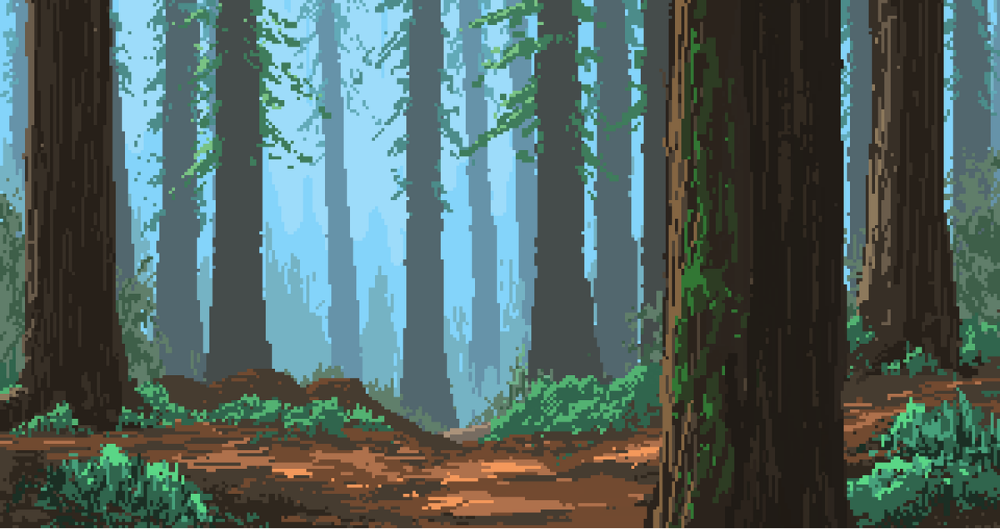
\includegraphics[width=0.3\linewidth]{images/dd_les.png}\hspace{0.5cm}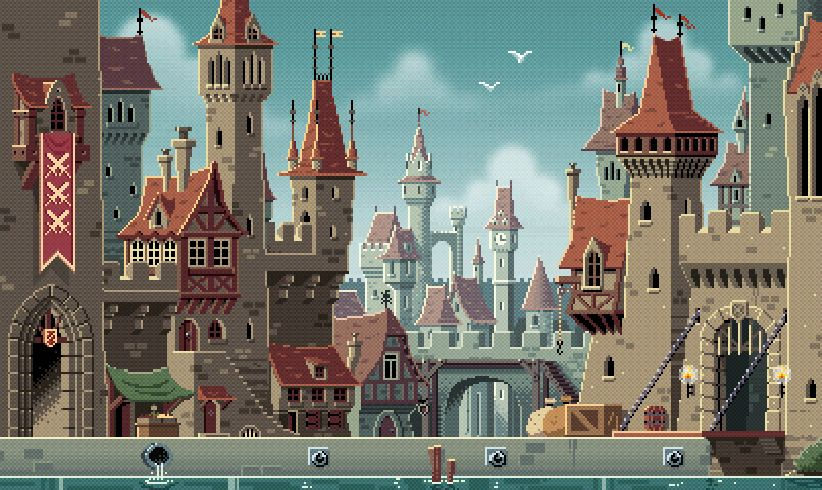
\includegraphics[width=0.3\linewidth]{images/dd_stolica.jpg}\hspace{0.5cm}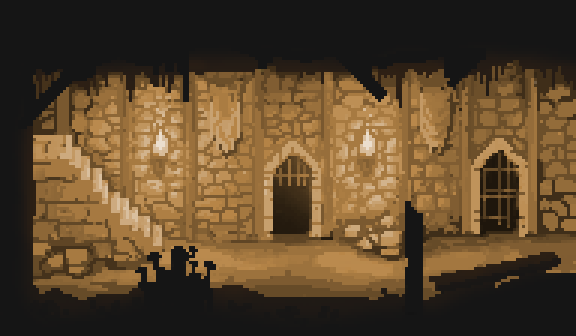
\includegraphics[width=0.3\linewidth]{images/dd_zamok.png}
\end{itemize}
\subsection{«Искусственный интеллект»}

\subsection{Многопользовательский режим}


\subsection{Интерфейс пользователя}
\subsubsection{Блок-схема}


\subsubsection{Функциональное описание и управление}


\subsubsection{Объекты интерфейса пользователя}


\subsection{Графика и видео}
\subsubsection{Общее описание}


\subsubsection{Двумерная графика и анимация}


\subsubsection{Трехмерная графика и анимация}


\subsubsection{Анимационные вставки}


\subsection{Звуки и музыка}
\subsubsection{Общее описание}


\subsubsection{Звук и звуковые эффекты}


\subsubsection{Музыка}


\subsection{Описание уровней}
\subsubsection{Общее описание дизайна уровней}


\subsubsection{Диаграмма взаимного расположения уровней}


\subsubsection{График введения новых объектов}


\newpage

\section{Контакты}
Контактная информация для обратной связи.
\end{document}
